\chapter{Surrogate based shape optimization}
\label{optimization}
The usual way of doing any CFD geometry optimization is shown in ~\ref{Closed Optimization loop}. But following this procedure is not feasible because it takes a lots of computational effort and time. Also, grid influences the solution considerably. So, using this method we can no longer guarantee that the changes in the solution of objective function value is because of the changes in the parameters of CAD or if they are coming from changes in the grid. The solution for the problems can be answered by developing a surrogate model.
\begin{figure}[H]
	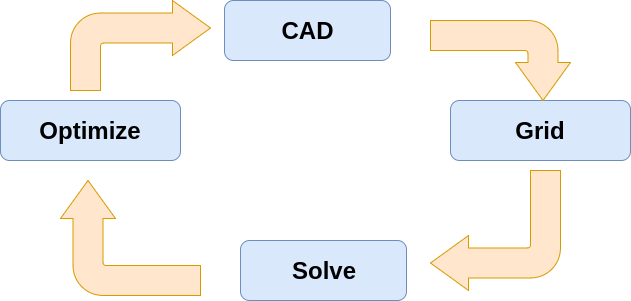
\includegraphics[width=\textwidth]{optimization/closed_loop.png}
	\caption{Closed Optimization loop}
	\label{Closed Optimization loop} %      only if needed
\end{figure}

\section{Surrogate model}

 Surrogate model is one of the mathematical and statistical techniques used to develop adequate functional relationship between an objective function y(x) and the control or design variables $ x_1 , x_2 .... x_k $. In our case, The model acts like a black box for aerodynamic parameters. Given the set of design variables, the model should give volumetric drag coefficient as shown in Figure \ref{Surrogate model} . The work flow associated with the development of a surrogate model is shown in Figure ~\ref{fig:work flow for the development of a surrogate model} . To develop an accurate surrogate, we need to carry out large number of CFD simulations. Creating geometry every time and meshing them is possible but takes a lot of time. Instead we can automate all the processes right from geometry creation to meshing and solving. This has become possible with OpenFOAM\textsuperscript{\textregistered}.

\begin{figure}[H]
	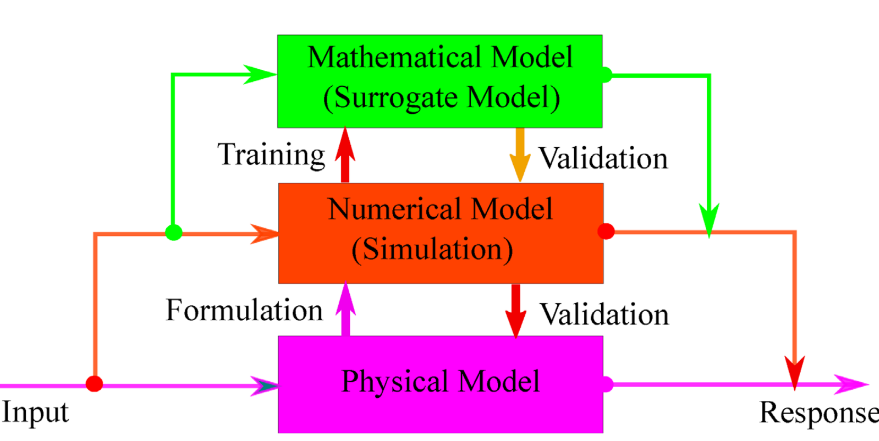
\includegraphics[width=\textwidth]{optimization/surrogate.png}
	\caption{Surrogate model definition}
	\label{Surrogate model} %      only if needed
\end{figure}

%\begin{figure}[htbp]
%	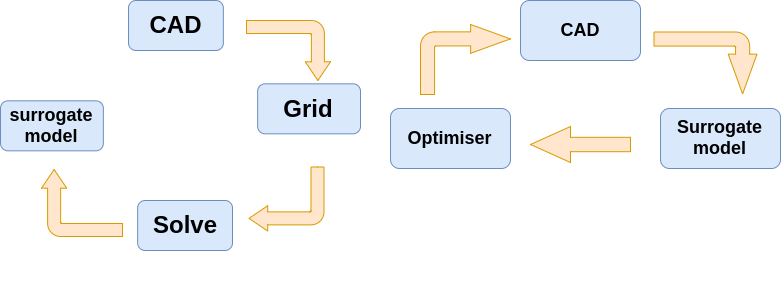
\includegraphics[width=\textwidth]{optimization/model.png}
%	\caption{Broken Optimization loop with the use of surrogate model}
%	\label{Broken Optimization loop with the use of surrogate model} %      only if needed 
%\end{figure}

\begin{figure}[htbp]
	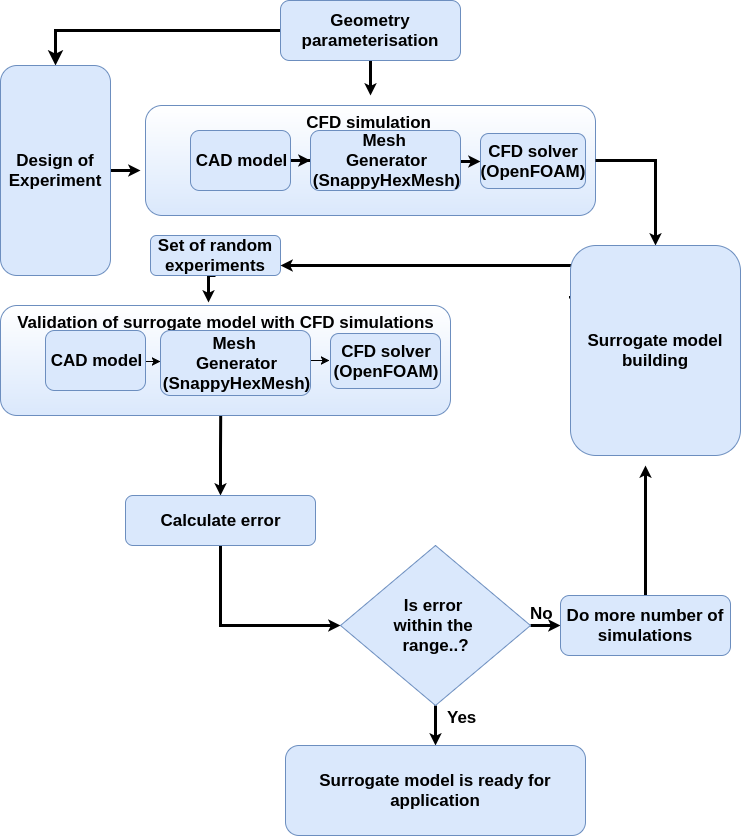
\includegraphics[width=\textwidth]{optimization/flow_chart.png}
  
	\caption{work flow for the development of a surrogate model}
	\label{fig:work flow for the development of a surrogate model} %      only if needed
\end{figure}


\section{Design of Experiments}

Design of Experiments is a technique used to extract maximum possible information from minimum number of computational experiments. This can be accomplished by the selection of a proper and robust scheme for DOE (Design of Experiments). In the present study, an open-source software named Surrogates Toolbox Version 3.0 (Viana, 2011) was used. Apart from many other important features, the toolbox provides an access to several varieties of widely used DOE models. Of the many DOE models available in the toolbox, optimal Latin Hypercube Sampling (OLHS) generated using translational propagation algorithm (TPA) \textbf{cite Viana et. al} was chosen, mainly due to its orthogonal structure. Fig. \ref{OLHS Sampling} shows sampling distribution of points in a unit square.

\begin{figure}[htbp]
	\centering
	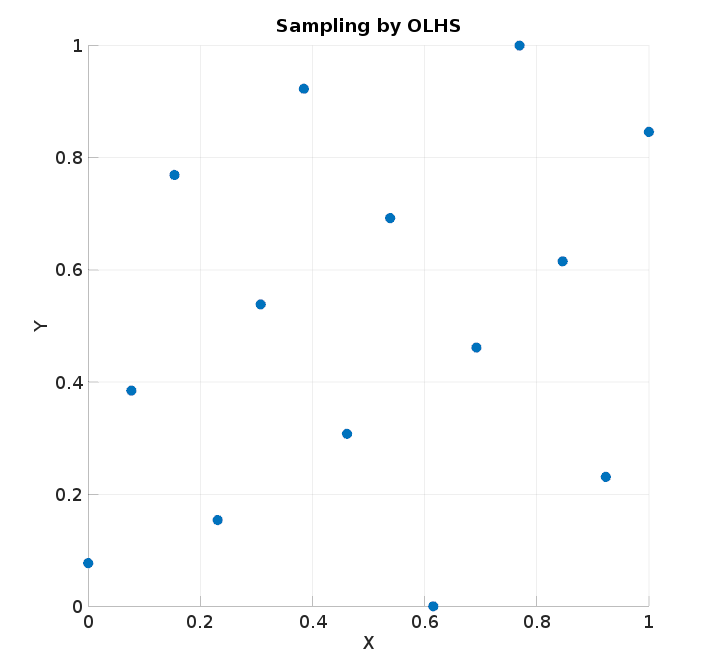
\includegraphics[width=200 pt]{optimization/OLHS_DOE}
	\caption{Sampling of unit square using OLHS }
	\label{OLHS Sampling}
\end{figure}

 The number of design experiments depends on the number of shape parameters used for defining geometry. A rule of thumb is that the number of design experiments should be ten times the number of shape parametres. However the actual number is decided by obtaining error between surrogate model results and actual CFD results. For the surrogate model to be acceptable, the error should be less than 2 percent. \cite{alam2016mdo} reported to have made 80 design experiments while developing his surrogate model for 2D bodies of revolution shapes. \cite{Kale2005a} reported to have studied about 600 feasible shapes using ANSYS\textsuperscript{\textregistered} \textit{Fluent} CFD package while developing quadratic response surface using Design Expert package.

For numerical experiments, Kriging surrogate model is reported to be best \citenum{viana2014metamodeling}. Kriging is named after the pioneering work of the South African mining engineer D. G. Krige. It is an interpolating method modelled by a Gaussian process governed by prior co-variances, which features the observed data at all design points. Kriging provides a statistic prediction of an unknown function by minimizing its Mean Squared Error (MSE).

The Kriging method in its basic formulation estimates the value of a function at some un sampled location as the sum of two components: the linear regression model $ f_i (x) $ (e.g., polynomial trend) of the data with p regressors modelling the drift of the process mean, i.e., the trend, over the domain, and a systematic departure representing low (large scale) and high frequency (small scale) variation components, respectively.

\section{Mapping design variables}
The first task before creation of DOE was the proper definition of the upper and lower limits for the six design variables (viz., $ m, r_0, r_1, C_p, \frac{l}{d} \ and \  scale \_y $). the design space is confined as mentioned in Table \ref{Degign space }

\begin{table}[H]
	\centering
	\caption{Design Space}
	\label{Degign space }
	%\begin{ruledtabular}
	\begin{tabular}{lll}
		\hline \hline
		Design Parameters & Min. & Max.    \\ \hline \hline
		
		$ Point\ of\ Max.\ Dia., m$ & 0.35 & 0.50     \\  
		$ Nose\ Radius, r _{o} $ & 0.20 & 0.80     \\
		$ Tail\ Radius, r _{1} $ & 0.1 & 0.5     \\  
		$ Prismatic\ Coeff., C _{p }$ & 0.55 & 0.70 \\
		$ Fineness\ Ratio, \frac{l}{d} $ &2.50 & 6.00 \\
		$Scaling\ in\ Y\ direction,\ scale\_y$ &1.00 & 5.00\\ \hline \hline
	\end{tabular}
	%	\end{ruledtabular}
\end{table}

Hundred candidate points were first obtained by Surrogates Toolbox \textbf{cite surrogate toolbox} using the Optimal Latin Hypercube Sampling (OLHS) method. The generated points were then mapped to the shapes corresponding to envelope volume ($ V _{env} $ ) of 250000 $ m^3 $ . .


\section{Test Function for Kriging Surrogate Model}
The Himmelblau function is taken as a test function.  It has one local maxima and four local minima in the domain x = [-6,6] and y = [-6,6]. The function is defined as 
\begin{equation}
f(x,y) = (x^2 + y - 11)^2  + (x + y^2 - 7)^2 
\end{equation}
\begin{equation}
x \in [-6,6] ;\quad y \in [-6,6]
\end{equation}

It has one local maximum at x=-0.270845 and y=-0.923039 where f(x,y)=181.617, and four identical local minima:
\begin{align}
&f( 3.0000 , 2.0000 )=0.0 \\
&f( -2.8051 , 3.1313 )=0.0 \\
&f( -3.7793 , -3.2831 )=0.0 \\
&f( 3.5844 , -1.8481 )=0.0 \\
\end{align}

If a small number of design points are used to create a surrogate model, then the approximate model created is prone to large errors at the trial points. However, the prediction accuracy of a surrogate model cannot be improved merely by taking larger number of design points; that is a function of its behaviour, design space and the required accuracy. Fig. \ref{fig:Root Mean Square Error with Design Points considered} shows the effect of increase in number of design points on the Root Mean Square Error (RMSE) of this test function. It is seen that the prediction accuracy of the model improves till 120 design points, after which addition of more design points does not approximate model for surrogate on the right with all the design points and test points. The actual value fo the function and predicted value from the surrogate model at test points are seen to match with each other within 1\%.

\begin{figure}[H]
	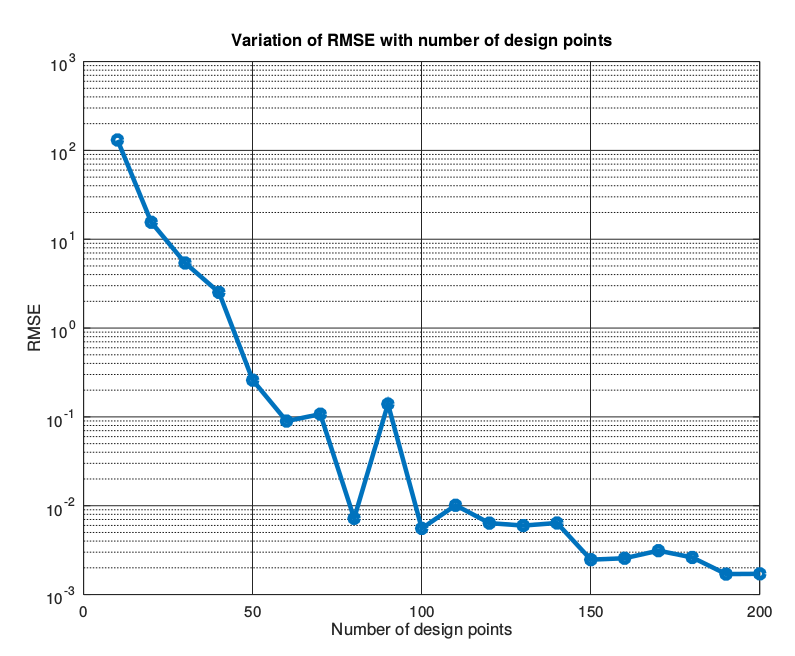
\includegraphics[width=\textwidth]{optimization/RMSE_analysis.png}
	\caption{Root Mean Square Error with Design Points considered}
	\label{fig:Root Mean Square Error with Design Points considered} %      only if needed
\end{figure}


\begin{figure}[H]
	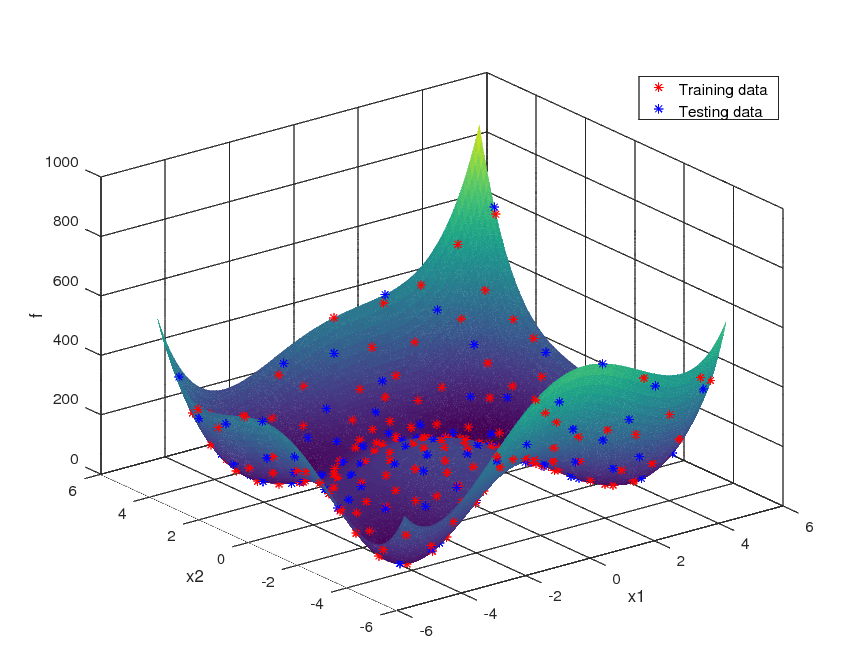
\includegraphics[width=\textwidth]{optimization/Himmel_blau_fcn.png}
	\caption{Comparison of Himmelblau function with its Surrogate Model}
	\label{fig:Comparison of Himmelblau function with its Surrogate Model} %      only if needed
\end{figure}

\section{Coupling of Genetic Algorithm, Surrogate model and testing for modified Himmelblau functions}
It is a well known fact that evolutionary algorithms like Genetic algorithm searches for global minimum and outputs that global minimum as final answer. Unlike gradient based methods, it should not get struck in local minimum. In order to check this, we modify the existing Himmelblau function. This is because actual Himmelblau function has four identical local minimum and don't have any global mimima. So, we modify it by adding the term $  0.01* (x + 3.7793)^2 + (y + 3.2832)^2 $. This term is added to the function value evaluated at all points except (-3.7793,-3.2832). Hence we obtained modified Himmelblau function with one global minima at (-3.7793,-3.2832) and three local minima at other three points. If we optimise this modified Himmelblau function using Genetic algorithm, we have to get the final answer as (-3.7793,-3.2832). The same answer is expected using surrogate model for the modified Himmelblau function. The obtained results are shown in Table.

\begin{table}[H]
	\centering
	\caption{Results obtained for modified Himmelblau function}
	\label{Results obtained for modified Himmelblau function}
	%\begin{ruledtabular}
	\begin{tabular}{llll}
		\hline \hline
		& X & Y & Function value \\ \hline
		Actual Function & -3.7793 &-3.2832 &1.6725e-11 \\
		Surrogate model & -3.7791 &-3.2828 & 2.5643e-03 \\ \hline
		\% error & 0.006 & 0.013 & 2.5643e-03 \\
		\hline \hline
		
		
		
		
	\end{tabular}
	%	\end{ruledtabular}
\end{table}






%%


%%% Local Variables: 
%%% mode: latex
%%% TeX-master: "../mainrep"
%%% End: 
